\section{Forward Surrogates: Two Resonators}

All ten forward architectures are trained on the same dataset, 100{,}000 configurations of two resonators each, for 200 epochs, and compared on the same 10{,}000-configuration test split. Table~\ref{tab:forward-results} reports the root-mean-square error (RMSE) between each model's predicted ERP spectrum and the solver's, the coefficient of determination ($R^2$), the Pearson correlation, and the RMSE restricted to the resonance peaks, which is usually the hardest part of the spectrum to get right. The architectures are listed in the same order throughout this chapter, with the plain feed-forward baseline NN last.

\begin{table}[h]
\centering
\caption[Forward surrogate comparison on the test split]{Forward architectures on the two-resonator test split (10{,}000 spectra). Lower RMSE and higher $R^2$ and Pearson $r$ are better.}
\label{tab:forward-results}
\begin{tabular}{lrrrrr}
\hline
Model & Parameters & RMSE (dB) & $R^2$ & Pearson $r$ & RMSE at peaks (dB) \\
\hline
DON   & 144{,}756 & 3.939 & 0.8369 & 0.9405 & 7.151 \\
DNO   & 143{,}434 & 1.212 & 0.9846 & 0.9924 & 3.841 \\
DCO   & 147{,}094 & 1.113 & 0.9870 & 0.9936 & 3.706 \\
SIREN & 145{,}820 & 1.538 & 0.9752 & 0.9879 & 4.315 \\
FNO   & 145{,}050 & 1.834 & 0.9646 & 0.9841 & 5.278 \\
WNO   & 146{,}318 & 1.956 & 0.9598 & 0.9818 & 6.557 \\
LNO   & 144{,}199 & 1.430 & 0.9785 & 0.9896 & 4.230 \\
GNO   & 143{,}718 & 2.107 & 0.9533 & 0.9805 & 4.801 \\
STO   & 144{,}213 & 2.096 & 0.9538 & 0.9799 & 4.894 \\
NN    & 144{,}481 & 6.241 & 0.5907 & 0.8417 & 11.747 \\
\hline
\end{tabular}
\end{table}

DCO and DNO, the two architectures developed specifically for this thesis, come out ahead of the others, with DCO reaching about 1.1\,dB RMSE on unseen designs. LNO and SIREN follow, FNO, WNO, STO and GNO lie between 1.8 and 2.1\,dB, and DON reaches 3.9\,dB. The plain feed-forward baseline, NN, is clearly the weakest, which confirms that giving the network an explicit, permutation-invariant encoder for the resonator set and physics-aware frequency features, which every other architecture uses and NN does not, is worth the added complexity.

The averages hide how the errors are distributed over the test split. Computed per spectrum, the median RMSE of DCO is only 0.82\,dB, and for every architecture except DON and NN at most 0.5\,\% of the test spectra have an RMSE above 5\,dB (13.8\,\% for DON and 88.4\,\% for NN). Figure~\ref{fig:forward-best-2res} shows, for each architecture, the test spectrum it predicts best. Every architecture except NN reproduces the solver curve almost exactly, with an RMSE between 0.2 and 1.2\,dB (3.6\,dB for NN). In most of these cases (seven of the ten) at least one resonator is tuned below the first plate resonance at about 54\,Hz, where it hardly changes the response, so the spectrum stays close to that of the bare plate and is easy to learn. Figure~\ref{fig:forward-worst-2res} shows the opposite end, the test spectrum each architecture predicts worst. The errors there range from 5.4\,dB (WNO) to 9.4\,dB (DON), and 11.8\,dB for NN, and they arise in the same place: the two resonators are tuned in the upper part of the band, mostly above 120\,Hz and often within a few hertz of each other, where the resonance peaks are narrow and overlap, so the predictions smooth them out or place them at slightly wrong frequencies. In most of these worst cases one resonator also sits close to the force position, where it couples most strongly to the plate. Even then, the first plate resonances at lower frequencies are reproduced well by every architecture except NN.

\begin{figure}[p]
\centering
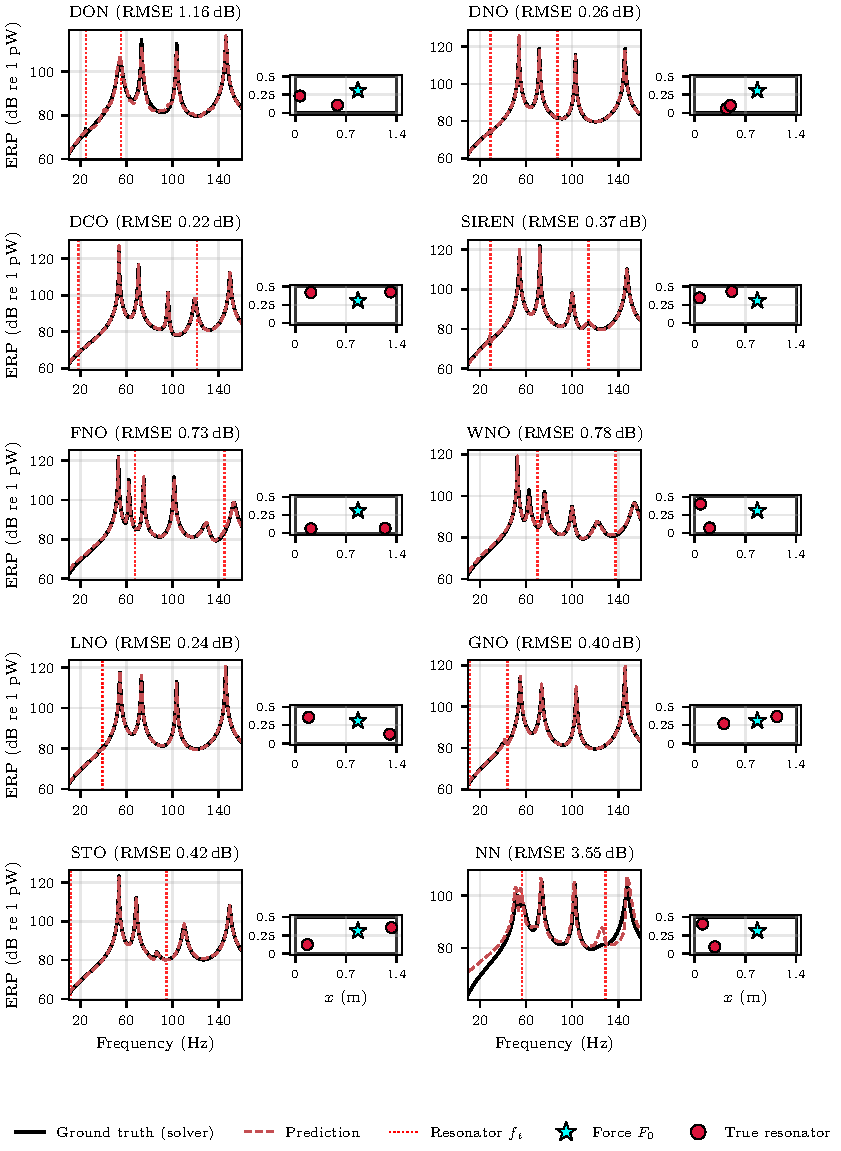
\includegraphics[max width=\textwidth,max height=0.84\textheight]{Bilder/forward_models_best_case_two_resonators.pdf}
\caption[Best test spectrum of each forward architecture, two resonators]{Best case of each forward architecture on the two-resonator test split: the test spectrum with the lowest RMSE, solver (black) against prediction (red dashed), with the resonator layout of that spectrum on the plate next to it.}
\label{fig:forward-best-2res}
\end{figure}

\begin{figure}[p]
\centering
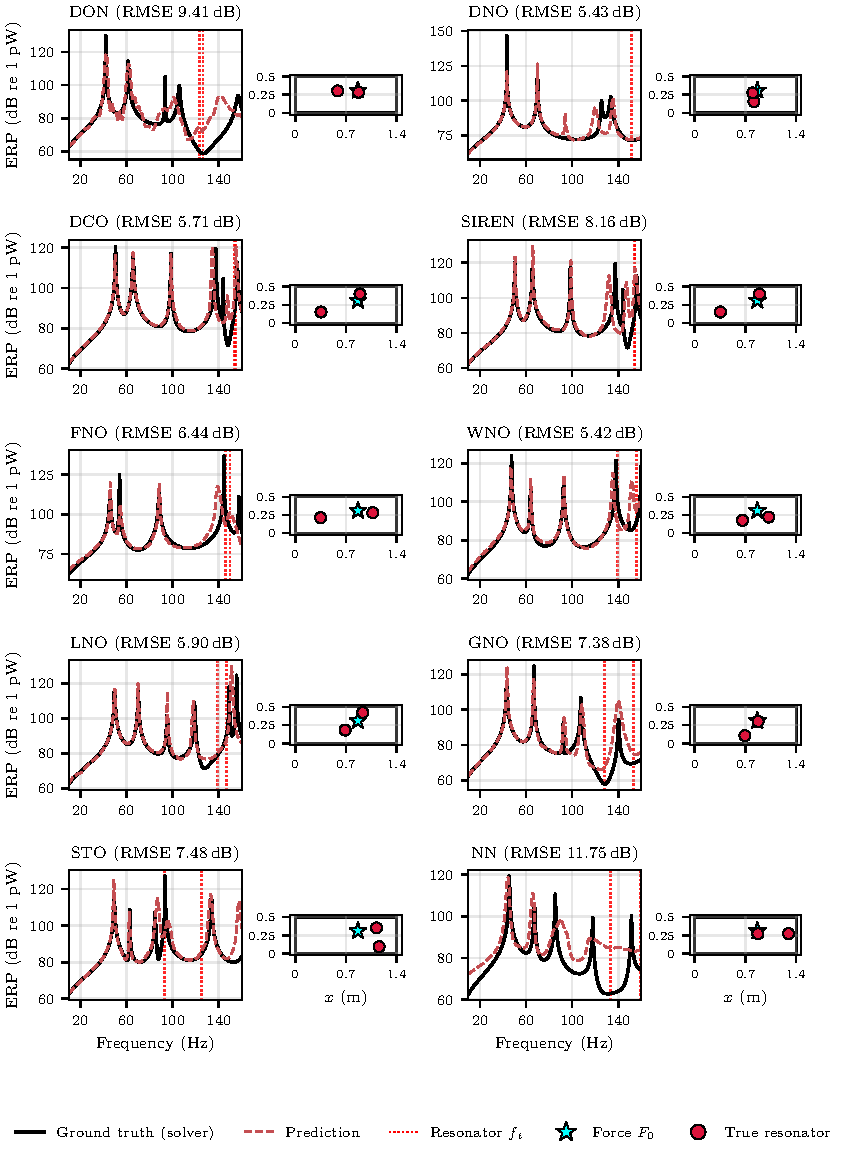
\includegraphics[max width=\textwidth,max height=0.84\textheight]{Bilder/forward_models_worst_case_two_resonators.pdf}
\caption[Worst test spectrum of each forward architecture, two resonators]{Worst case of each forward architecture on the two-resonator test split: the test spectrum with the highest RMSE. The largest disagreements occur at resonances in the upper part of the band, where the two tuned resonators lie close together.}
\label{fig:forward-worst-2res}
\end{figure}

Figure~\ref{fig:dco-parity} (left) shows DCO's predictions against the solver's values across the whole two-resonator test split: the points follow the ideal line closely over the whole range of ERP values ($R^2 = 0.987$), with the spread growing at the highest ERP values, which occur at the resonance peaks.

\begin{figure}[h]
\centering
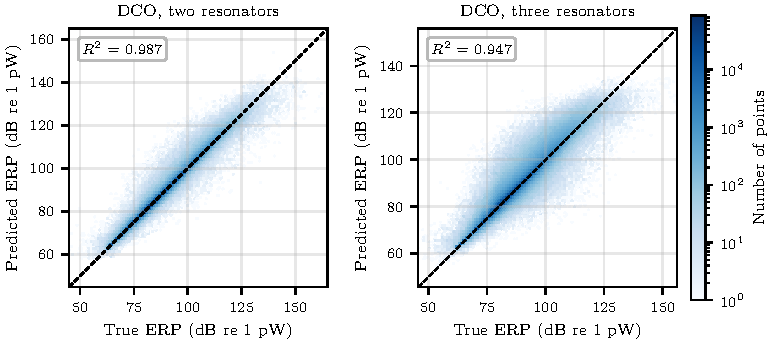
\includegraphics[max width=\textwidth]{Bilder/forward_dco_prediction_vs_true_erp.pdf}
\caption[DCO predicted versus true ERP]{DCO: predicted ERP against the solver's ERP, across the full test split of the two-resonator (left) and the three-resonator (right) dataset. Colour shows the number of points per cell on a logarithmic scale.}
\label{fig:dco-parity}
\end{figure}

\section{Forward Surrogates: Three Resonators}
\label{sec:results-3res}

The same ten architectures are also compared on a three-resonator dataset of 100{,}000 configurations. It is generated exactly like the two-resonator dataset: the same plate, the same 18 plate modes ($6\times3$), and the same five-variable design space with a sampled damping ratio; only the number of resonators per configuration changes. Table~\ref{tab:forward-results-3res} reports the same metrics as Table~\ref{tab:forward-results}.

\begin{table}[h]
\centering
\caption[Forward surrogate comparison, three resonators]{Forward architectures on the three-resonator test split (10{,}000 spectra, 18 plate modes).}
\label{tab:forward-results-3res}
\begin{tabular}{lrrrrr}
\hline
Model & Parameters & RMSE (dB) & $R^2$ & Pearson $r$ & RMSE at peaks (dB) \\
\hline
DON   & 151{,}560 & 4.677 & 0.7593 & 0.9104 & 8.139 \\
DNO   & 150{,}238 & 2.271 & 0.9432 & 0.9735 & 5.252 \\
DCO   & 155{,}536 & 2.186 & 0.9474 & 0.9753 & 5.238 \\
SIREN & 153{,}002 & 2.481 & 0.9322 & 0.9690 & 5.516 \\
FNO   & 153{,}870 & 2.773 & 0.9153 & 0.9594 & 6.510 \\
WNO   & 153{,}626 & 3.046 & 0.8979 & 0.9530 & 7.324 \\
LNO   & 152{,}011 & 2.688 & 0.9205 & 0.9642 & 5.781 \\
GNO   & 143{,}718 & 2.659 & 0.9222 & 0.9690 & 4.874 \\
STO   & 144{,}213 & 2.930 & 0.9055 & 0.9626 & 5.308 \\
NN    & 145{,}489 & 7.159 & 0.4358 & 0.7980 & 12.581 \\
\hline
\end{tabular}
\end{table}

The top and the bottom of the ranking are the same as in the two-resonator case: DCO and DNO still lead, with 2.19\,dB and 2.27\,dB, and NN and DON are still the weakest. In the middle the order changes: SIREN stays close behind the two leaders, GNO moves from eighth to fourth place, and with 4.87\,dB it now has the lowest RMSE at the resonance peaks of all ten architectures, although its overall RMSE is only middling. What changes most is the overall difficulty: the RMSE of the best architectures roughly doubles going from two to three resonators (DCO from 1.11\,dB to 2.19\,dB, DNO from 1.21\,dB to 2.27\,dB, LNO from 1.43\,dB to 2.69\,dB), while the weaker architectures increase less (DON from 3.94\,dB to 4.68\,dB, NN from 6.24\,dB to 7.16\,dB). Overall the increase is a factor of 1.1 to 2.0. With a third resonator there are more mode shapes to couple to, more possible near-coincidences between tuning frequencies, and a higher-dimensional design to encode, so this increase is expected. That the best and the worst architectures stay the same under a harder problem is evidence that the comparison in Table~\ref{tab:forward-results} reflects a real property of each architecture, not an artefact of the easier two-resonator case. The right panel of Figure~\ref{fig:dco-parity} shows the same effect for DCO: the $R^2$ drops from 0.987 to 0.947 and the cloud around the ideal line widens.

Figure~\ref{fig:forward-best-3res} and Figure~\ref{fig:forward-worst-3res} show the best and the worst test spectrum of every architecture, as for two resonators. In the best cases every architecture except NN is within 1.4\,dB of the solver (NN: 3.6\,dB), and every one of these configurations has at least one resonator tuned below the first plate resonance. The worst cases reach 8.3 to 11.6\,dB (12.7\,dB for NN), again with resonators tuned in the upper half of the band, and they are largely shared between architectures: SIREN, FNO, GNO and STO all fail most on the same configuration (tuning frequencies of about 106, 148 and 154\,Hz), DNO and WNO fail most on another one (131, 140 and 151\,Hz), and DON and NN on a third. A configuration that is hard for one architecture is therefore usually hard for the others as well, which points to the physics of closely spaced, strongly coupled resonances rather than to a weakness of any single architecture. Only 1.6 to 4.2\,\% of the test spectra of DNO, DCO, SIREN, FNO, WNO, LNO, GNO and STO have an RMSE above 5\,dB, against 31.8\,\% for DON and 98.7\,\% for NN.

\begin{figure}[p]
\centering
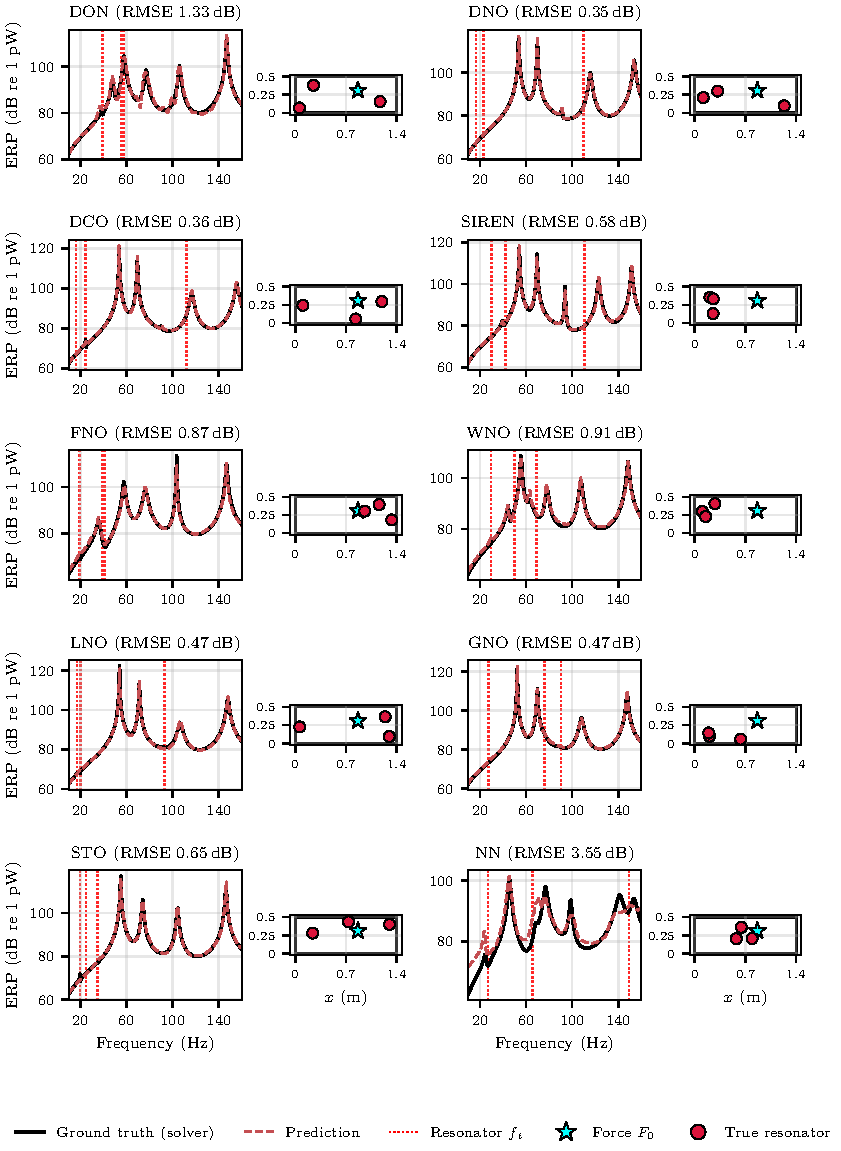
\includegraphics[max width=\textwidth,max height=0.84\textheight]{Bilder/forward_models_best_case_three_resonators.pdf}
\caption[Best test spectrum of each forward architecture, three resonators]{Best case of each forward architecture on the three-resonator test split, in the same format as Figure~\ref{fig:forward-best-2res}.}
\label{fig:forward-best-3res}
\end{figure}

\begin{figure}[p]
\centering
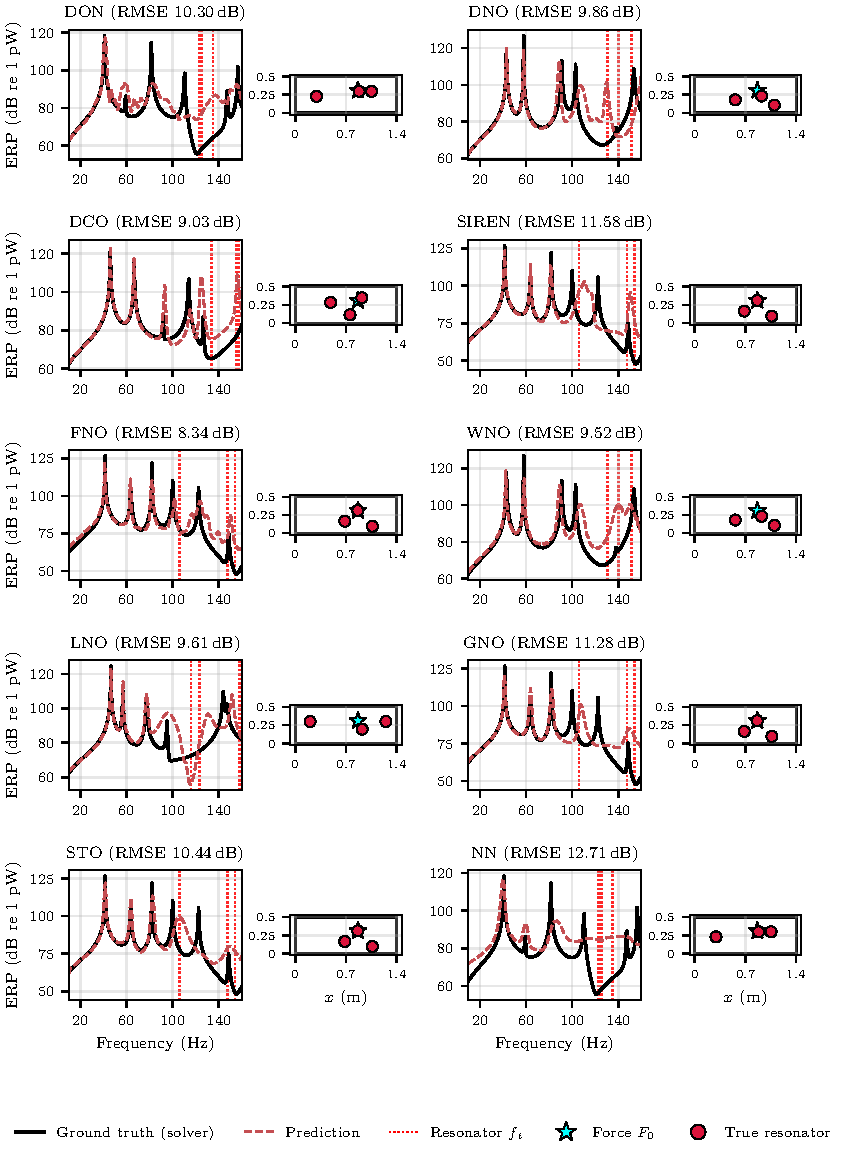
\includegraphics[max width=\textwidth,max height=0.84\textheight]{Bilder/forward_models_worst_case_three_resonators.pdf}
\caption[Worst test spectrum of each forward architecture, three resonators]{Worst case of each forward architecture on the three-resonator test split. Several architectures fail on the same configurations, where resonators are tuned in the upper part of the band.}
\label{fig:forward-worst-3res}
\end{figure}

\section{Invertible Operators and Generative Design}

The invertible architectures described in Section~\ref{sec:idon} and Section~\ref{sec:ifno} are evaluated on the earlier, 200{,}000-configuration two-resonator dataset introduced there (four design variables per resonator, fixed damping), on its test split of 20{,}000 configurations. For every target spectrum, each invertible model proposes 8 candidate designs; three selection rules are then scored against the solver's own response to the proposed design: a random one of the 8 samples, the sample the model itself would predict is closest to the target (without using the target), and an oracle that picks the closest of the 8 to the true target (an upper bound, since it uses the target). Table~\ref{tab:inverse-ifno} reports the forward accuracy of all invertible models together with their own-forward-selected inverse accuracy for 100 target spectra, and how well they recover two representative design variables: the tuning frequency, which turns out to be the best-recovered variable, and the $y$ position, which turns out to be the hardest. Note that iDNO and iDCO were trained with a shorter schedule than the other family members (Section~\ref{sec:training}).

\begin{table}[h]
\centering
\caption[Invertible operator comparison]{The invertible architectures on the 200{,}000-configuration two-resonator dataset: forward accuracy on the 20{,}000-configuration test split, own-forward-selected inverse accuracy (solver-checked, 100 target spectra, 8 samples each), and design-recovery correlation for the best- and worst-recovered variable. iDON (Q8) is the unpadded variant of Section~\ref{sec:idon}.}
\label{tab:inverse-ifno}
\small
\setlength{\tabcolsep}{4pt}
\begin{tabular}{lrrrrrrr}
\hline
Model & Parameters & Fwd RMSE (dB) & Fwd $R^2$ & Inv RMSE (dB) & Inv $r$ & $r(f_t)$ & $r(y)$ \\
\hline
iDON (Q64) & 1{,}384{,}257 & 2.673 & 0.9301 & 5.779 & 0.836 & 0.906 & 0.224 \\
iDON (Q8)  & 938{,}665 & 6.047 & 0.6423 & 10.077 & 0.500 & 0.803 & -0.055 \\
iDNO       & 84{,}389 & 2.698 & 0.9288 & 8.064 & 0.677 & 0.915 & 0.256 \\
iDCO       & 81{,}909 & 2.575 & 0.9351 & 7.791 & 0.698 & 0.909 & 0.123 \\
iFNO       & 188{,}405 & 2.371 & 0.9450 & 7.765 & 0.701 & 0.869 & 0.253 \\
iLNO       & 83{,}229 & 2.369 & 0.9451 & 7.930 & 0.687 & 0.902 & 0.151 \\
iGNO       & 62{,}210 & 3.773 & 0.8608 & 8.065 & 0.675 & 0.914 & 0.154 \\
iSTO       & 71{,}089 & 2.556 & 0.9361 & 7.833 & 0.695 & 0.914 & 0.225 \\
\hline
\end{tabular}
\end{table}

Three things stand out. First, the forward accuracy of the invertible architectures, 2.4 to 3.8\,dB for the six family members and 2.7\,dB for iDON (Q64), is lower than that of the plain forward architectures on the two-resonator dataset of Table~\ref{tab:forward-results} (1.1 to 2.1\,dB for eight of the ten), and it is comparable to them on the harder three-resonator dataset of Table~\ref{tab:forward-results-3res} (2.2 to 3.0\,dB for eight of the ten). The datasets are not identical (200{,}000 configurations with fixed damping against 100{,}000 with sampled damping), so this comparison is only indicative, but it suggests that making a core invertible does cost some forward accuracy, which is the price of also getting the inverse direction from the same weights. The family members have between 62{,}000 and 188{,}000 parameters, against about 145{,}000 for each forward architecture, while iDON, whose branch and trunk networks are much wider, has 1.4 million. Figure~\ref{fig:idon-forward-parity} shows the forward half directly for iDON (Q64): predicted against true ERP across the whole test split. The points follow the ideal line over most of the range ($R^2 = 0.930$), but the predictions flatten out above about 110\,dB, so the highest resonance peaks are systematically underestimated.

\begin{figure}[h]
\centering
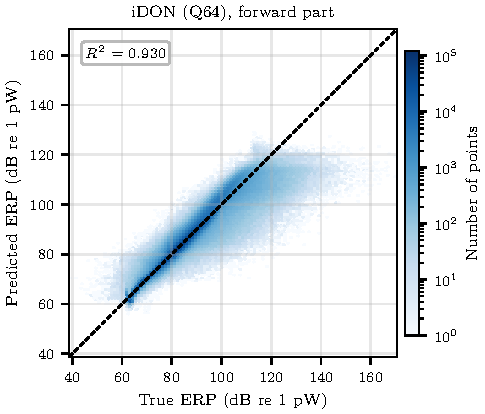
\includegraphics[max width=\textwidth]{Bilder/idon_forward_prediction_vs_true_erp.pdf}
\caption[iDON forward predicted versus true ERP]{iDON (Q64, forward direction): predicted ERP against the solver's ERP, across the full test split of the 200{,}000-configuration dataset.}
\label{fig:idon-forward-parity}
\end{figure}

Figure~\ref{fig:invertible-best} and Figure~\ref{fig:invertible-worst} show the best and the worst test spectrum of each invertible model in the forward direction. In the best cases all models follow the solver closely (RMSE 0.6 to 1.1\,dB, 1.9\,dB for iDON (Q8)). In the worst cases the errors are 6.0\,dB for iDON (Q64), 6.7 to 9.3\,dB for the family and 13.7\,dB for iDON (Q8); the largest deviations occur where the solver curve has several narrow, closely spaced peaks, as for the forward architectures, and in several of them a resonator sits right next to the force position.

\begin{figure}[p]
\centering
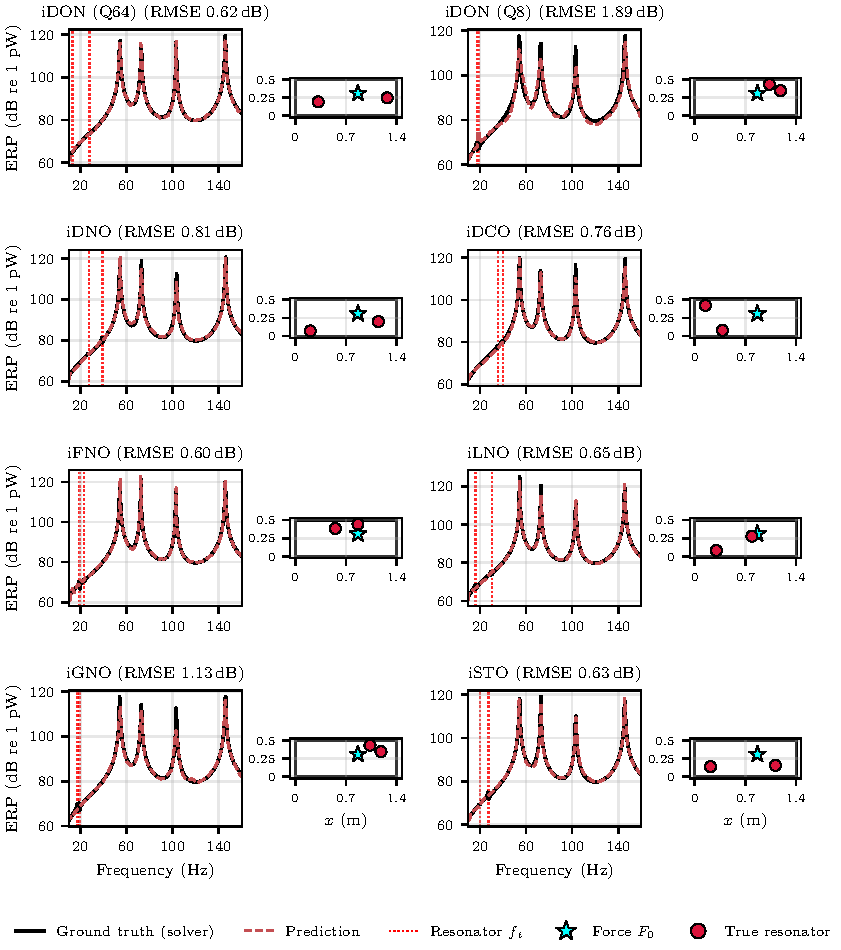
\includegraphics[max width=\textwidth,max height=0.84\textheight]{Bilder/invertible_models_forward_best_case.pdf}
\caption[Best forward prediction of each invertible model]{Forward direction of the invertible models on the 200{,}000-configuration dataset: for each model, the test spectrum with the lowest RMSE.}
\label{fig:invertible-best}
\end{figure}

\begin{figure}[p]
\centering
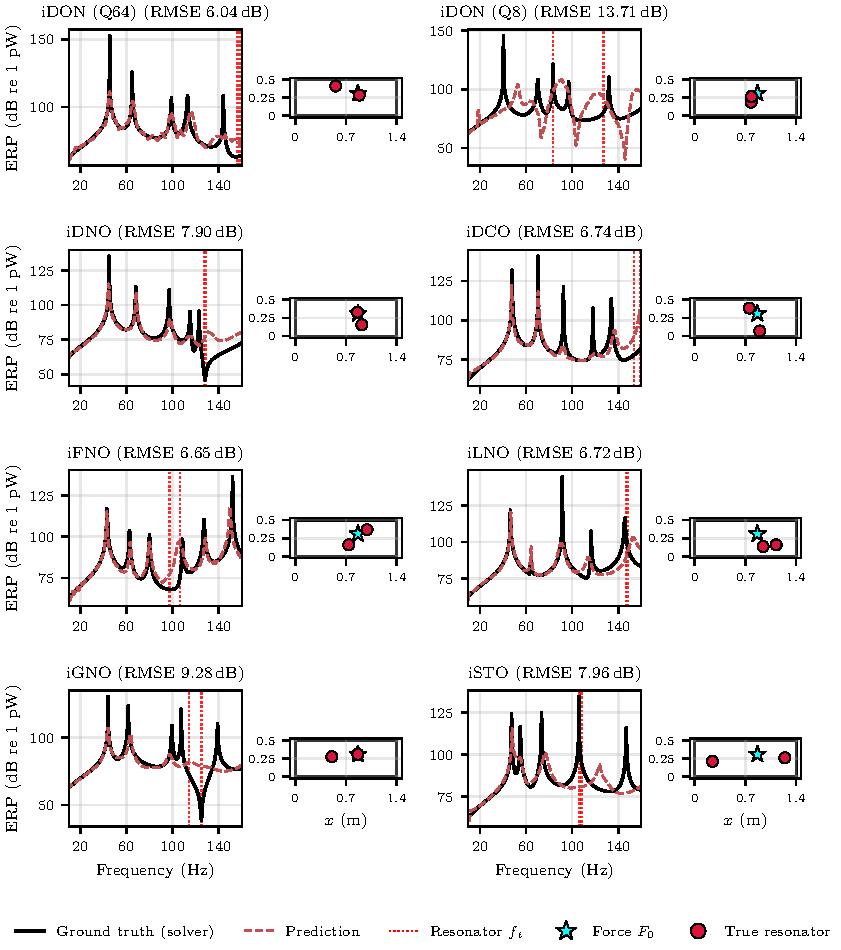
\includegraphics[max width=\textwidth,max height=0.84\textheight]{Bilder/invertible_models_forward_worst_case.pdf}
\caption[Worst forward prediction of each invertible model]{Forward direction of the invertible models on the 200{,}000-configuration dataset: for each model, the test spectrum with the highest RMSE.}
\label{fig:invertible-worst}
\end{figure}

Second, the inverse accuracy is far behind the forward accuracy for every model: around 7.8 to 8.1\,dB for the family instead of 2.4 to 3.8\,dB, and 5.8\,dB for iDON (Q64), the best inverse model, which is also the largest. The tuning frequency is recovered much better ($r(f_t)$ between 0.87 and 0.92) than the $y$ position ($r(y)$ between 0.12 for iDCO and 0.26 for iDNO). This matches the non-uniqueness argument made in Chapter~\ref{ch:theory}: many different resonator positions can produce a very similar spectrum, especially along the plate's short, 0.5\,m $y$ direction, so recovering a spectrum's tuning frequencies is a much better-posed problem than recovering exact positions. Figure~\ref{fig:ifno-inverse-example} shows the same target spectrum and the proposal selected by each model's own forward direction, together with the true and the proposed resonator positions on the plate. Every model reproduces the general rising shape of the spectrum and lines up with the target at several resonance peaks, but every model also proposes extra peaks the target does not have and misses others: iDON (Q64) matches almost all peaks (3.9\,dB), apart from one spurious peak near 33\,Hz, the family members reach 6.1 to 9.1\,dB, and iDON (Q8) fails to reproduce the spectrum (12.3\,dB). The plate in the lower panel shows why the proposals differ from the truth: most proposed resonators lie in the neighbourhood of the force and of the first true resonator, none of them is placed near the second true resonator at the lower plate edge, and almost all proposed positions lie between $y = 0.2$ and $0.35$\,m, around the centre line of the plate.

\begin{figure}[p]
\centering
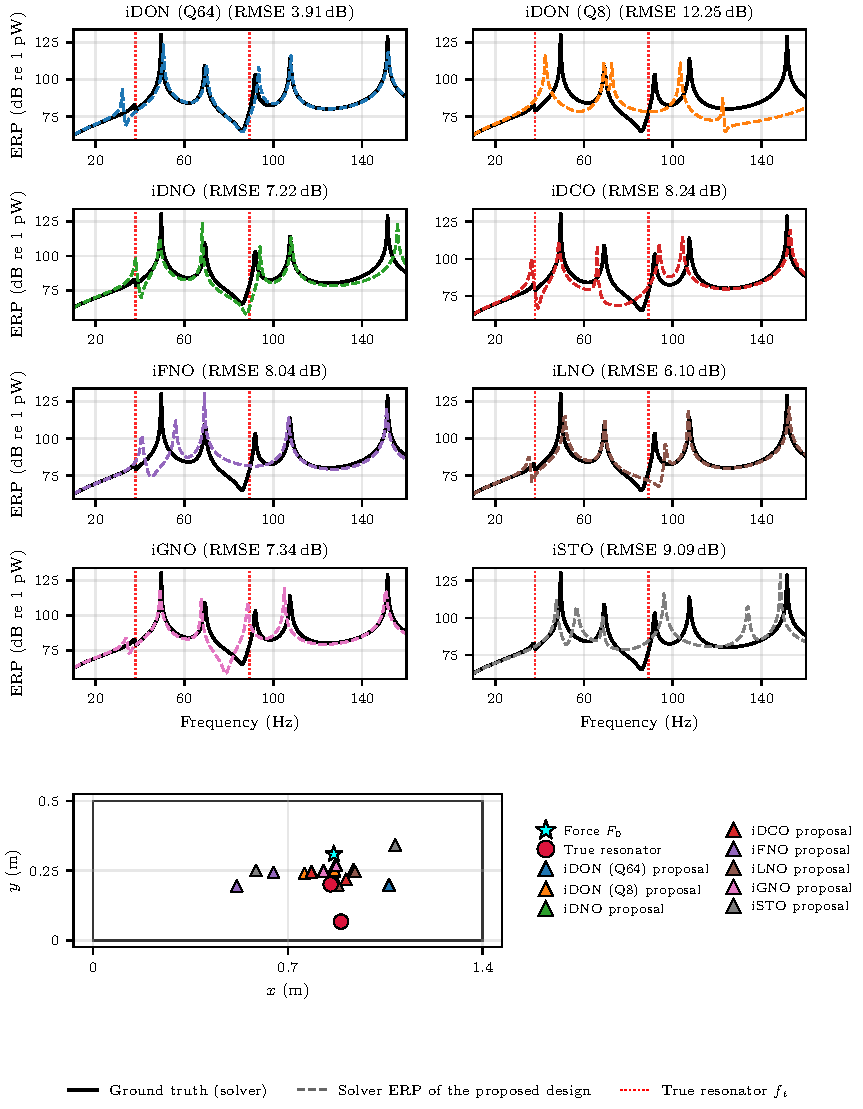
\includegraphics[max width=\textwidth,max height=0.84\textheight]{Bilder/invertible_models_inverse_prediction.pdf}
\caption[Inverse design example, all invertible models]{One target spectrum (black) and the proposal selected by the own forward direction (coloured, 8 samples per model) from all invertible models, re-simulated with the solver. The plate shows the two true resonators (red circles) and the proposed resonators of every model (triangles in the colour of the model).}
\label{fig:ifno-inverse-example}
\end{figure}

Figure~\ref{fig:idon-inverse-parameters} shows the same weakness over many targets, for iDON (Q64): for 4{,}000 test targets, the proposed value of each design variable against the true one. The tuning frequency lies on the diagonal ($r = 0.87$) and the $x$ position follows it clearly ($r = 0.69$), whereas the mass is only loosely recovered ($r = 0.40$) and the $y$ position collapses onto a narrow band around $y \approx 0.25$\,m ($r = 0.29$): the model proposes a $y$ position near the plate's centre line almost regardless of the target, presumably because the spectrum constrains it only weakly.

\begin{figure}[h]
\centering
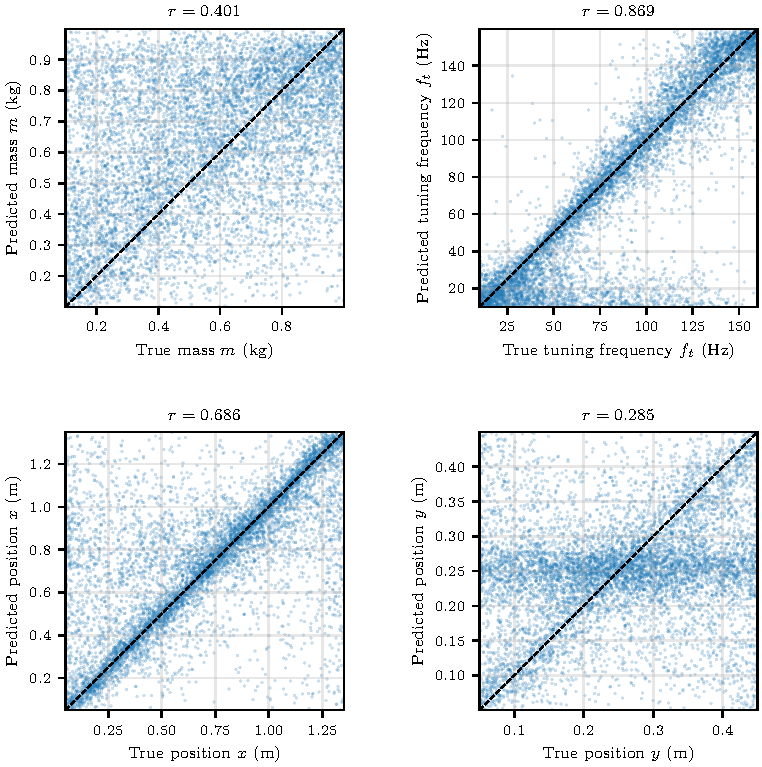
\includegraphics[max width=\textwidth]{Bilder/idon_inverse_prediction_vs_true_parameters.pdf}
\caption[iDON: predicted versus true resonator parameters]{iDON (Q64, inverse direction): proposed against true resonator parameters for 4{,}000 test targets (one sample per target, selected by the model's own forward direction; resonators ordered by tuning frequency).}
\label{fig:idon-inverse-parameters}
\end{figure}

Third, iDON is evaluated separately, since its design-size parameter $Q$ is itself a modelling choice, discussed in Section~\ref{sec:idon}. Table~\ref{tab:idon-q} confirms the effect of padding beyond the design size $D=8$ numerically: Q64 is clearly better than Q8 on every metric, including the position-recovery error, which is reported directly in centimetres rather than as a correlation, and which is roughly halved. One caveat applies to this comparison: the Q8 training run stopped early, after 50 of the 150 planned epochs (Section~\ref{sec:training}), so part of its disadvantage may come from the shorter training and not from the missing padding alone.

\begin{table}[h]
\centering
\caption[iDON: Q8 versus Q64]{iDON with the design-sized basis (Q8, $Q=D=8$) against the padded basis (Q64, $Q=64$): inverse results for 500 test targets, 16 samples each (selected by the own forward direction); the forward RMSE is that of the full test split.}
\label{tab:idon-q}
\begin{tabular}{lrrrr}
\hline
Variant & Fwd RMSE (dB) & Inv RMSE (dB) & $r(f_t)$ & Median position error (cm) \\
\hline
Q8  & 6.047 & 9.969 & 0.812 & 24.4 \\
Q64 & 2.673 & 5.165 & 0.867 & 12.8 \\
\hline
\end{tabular}
\end{table}

Taken together, these results show that the forward half of every invertible architecture works reasonably well, although less accurately than a dedicated forward architecture, and that the inverse direction already recovers the overall shape of a target spectrum and its dominant tuning frequencies reasonably well, while exact position recovery remains the hardest part of generative design with this approach, a limitation discussed further in Chapter~\ref{ch:conclusions}.
